\documentclass[11pt,a4paper]{article}

  \usepackage[utf8]{inputenc}
  \usepackage[T1]{fontenc}
  \usepackage[provide=*,italian]{babel}
  \usepackage{multirow}
  \usepackage[a4paper,margin=2.3cm,top=2.5cm,bottom=2.5cm]{geometry}
  \usepackage{setspace}
  \setstretch{1.15}
  \usepackage{parskip}
  \usepackage{xcolor}
  \definecolor{accent}{HTML}{0B5C8C}
  \definecolor{accent2}{HTML}{2E7D32}
  \definecolor{rowAlt}{HTML}{F5F7FA}
  \definecolor{headerBg}{HTML}{0B5C8C}
  \definecolor{warn}{HTML}{B71C1C}
  \usepackage[colorlinks=true,linkcolor=accent,urlcolor=accent,citecolor=accent]{hyperref}
  \usepackage{array}
  \usepackage{booktabs}
  \usepackage{longtable}
  \usepackage{tabularx}
  \usepackage{colortbl}
  \renewcommand{\arraystretch}{1.25}
  \usepackage{enumitem}
  \setlist[itemize]{itemsep=2pt,topsep=4pt,leftmargin=*}
  \setlist[enumerate]{itemsep=2pt,topsep=4pt,leftmargin=*}
  \usepackage{titlesec}
  \titleformat{\section}{\Large\bfseries\color{accent}}{\thesection}{0.6em}{}
  \titleformat{\subsection}{\large\bfseries\color{accent}}{\thesubsection}{0.5em}{}
  \titlespacing*{\section}{0pt}{18pt}{8pt}
  \titlespacing*{\subsection}{0pt}{12pt}{6pt}
  \usepackage{fancyhdr}
  \pagestyle{fancy}
  \fancyhf{}
  \fancyhead[L]{\small\textcolor{accent}{\textbf{Trento Live Activity}}}
  \fancyhead[R]{\small Milestone \#3, Sprint \#1}
  \fancyfoot[C]{\thepage}
  \renewcommand{\headrulewidth}{0.4pt}
  \usepackage{pgfplots}
  \pgfplotsset{compat=1.18}
  \usepackage{tikz}
  \usepackage{tcolorbox}
  \tcbset{
    callout/.style={
      colback=accent!5, colframe=accent, sharp corners,
      boxrule=0.5pt, left=8pt, right=8pt, top=6pt, bottom=6pt,
      fontupper=\small
    }
  }
  \newcommand{\code}[1]{\texttt{\small#1}}

  \begin{document}

  \begin{titlepage}
  \centering
  \vspace*{2cm}
  {\Huge\bfseries\color{accent} Trento Live Activity\par}
  \vspace{0.4cm}
  {\Large Report Milestone \#3, Sprint \#1\par}
  \vspace{1.5cm}
  \rule{0.6\textwidth}{0.4pt}\par
  \vspace{0.6cm}
  {\large Universit\`{a} degli Studi di Trento\par}
  {\large Dipartimento di Ingegneria e Scienza dell'Informazione (DISI)\par}
  {\large Corso di \emph{Software Engineering}, a.a. 2025--2026\par}
  \vspace{0.4cm}
  {\large Docente: Prof.\ Sandro Fiore\par}
  \vspace{1.5cm}
  \rule{0.6\textwidth}{0.4pt}\par
  \vspace{2cm}
  {\large\bfseries Gruppo 7\par}
  \vspace{0.3cm}
  \begin{tabular}{l}
  Anas Soussane, 243731 \\
  Filippo Marcatili, 243199 \\
  Saif Safi, 245473 \\
  \end{tabular}
  \vfill
  {\large Deadline: 17 maggio 2026\par}
  \end{titlepage}

  \tableofcontents
  \newpage

  \section{Sezione introduttiva}

  \subsection{Team Members}
  La tabella seguente riporta i tre membri del gruppo con le informazioni principali.
  \begin{center}
  \begin{small}
  \begin{tabular}{>{\bfseries}l c l l}
  \toprule
  \rowcolor{headerBg}\color{white}\textbf{Nome e Cognome} & \color{white}\textbf{Matricola} &
  \color{white}\textbf{Account GitHub} & \color{white}\textbf{Area principale} \\
  \midrule
  Anas Soussane     & 243731 & \href{https://github.com/anass03}{anass03}       & Backend, autenticazione, sicurezza, notifiche, AI \\
  Filippo Marcatili & 243199 & \href{https://github.com/flippomar}{flippomar}   & Backend, autenticazione, dashboard, frontend \\
  Saif Safi         & 245473 & \href{https://github.com/elliott-dp}{elliott-dp} & Frontend, mappa MapLibre, UI/UX \\
  \bottomrule
  \end{tabular}
  \end{small}
  \end{center}

  \subsection{Project Idea}
  \textbf{Trento Live Activity} \`{e} una piattaforma civic-tech web che permette ai cittadini
  di Trento di esplorare in tempo reale i dati urbani (parcheggi, affollamento, eventi, punti di
  interesse) su una mappa interattiva, e di creare o partecipare ad attivit\`{a} sociali
  spontanee. Gli enti certificati possono pubblicare eventi verificati, mentre il Comune dispone
  di una dashboard analitica per monitorare l'attivit\`{a} urbana in modo aggregato.

  \subsection{Links}
  \begin{itemize}
    \item \textbf{Repository GitHub:} \url{https://github.com/flippomar/trento-live-activity}
    \item \textbf{Specifica OpenAPI 3.0 sorgente:} \url{https://github.com/flippomar/trento-live-activity/blob/main/docs/openapi.yaml} (72 endpoint)
  \end{itemize}

  \section{Sezione generale}

  \subsection{Strategia di branching}
  Abbiamo adottato una strategia ibrida basata su \textbf{GitHub Flow}, con una convenzione di
  naming legata agli sprint. Abbiamo escluso fin dall'inizio il master-only per poter fare peer
  review in modo sistematico.

  \paragraph{Branch principali:}
  \begin{itemize}
    \item \textbf{\code{main}}: branch stabile, sempre deployabile. Le modifiche entrano solo
    tramite Pull Request approvata da almeno un altro membro.
    \item \textbf{\code{sprint<N>/<feature>}}: branch di feature per lo sprint corrente.
    Alcuni esempi dallo Sprint \#1: \code{sprint1/backend-setup}, \code{sprint1/auth},
    \code{sprint1/db-and-activities}, \code{sprint1/2fa-setup},
    \code{sprint1/firebase-notifications}, \code{sprint1/firebase-frontend},
    \code{sprint1/email-notifications}, \code{sprint1/audit-push-events-fixes},
    \code{sprint1/frontend}, \code{sprint1/ai-gemini-and-fixes},
    \code{sprint1/security-hardening}, \code{sprint1/ux-and-db-improvements},
    \code{sprint1/fix-moderation-notifications}, \code{sprint1/fix-push-location},
    \code{sprint1/feature-fixes}, \code{sprint1/feature-restoring},
    \code{sprint1/final-touches}, \code{sprint1/sprint2-batch}.
    \item \textbf{\code{fix/<short-name>}}: bug fix puntuali (es. \code{fix/moderation-report}).
  \end{itemize}
  Durante lo Sprint \#1 abbiamo creato \textbf{19 feature branch} e mergiato
  \textbf{32 Pull Request} su \code{main}.

  \paragraph{Workflow tipico:}
  \begin{enumerate}
    \item Si crea il branch da \code{main} aggiornato e si procede con commit incrementali,
    usando messaggi in forma imperativa.
    \item Appena la feature \`{e} funzionante, si apre la PR su GitHub.
    \item Almeno un altro membro del team fa la code review (requisiti, test, convenzioni,
    sicurezza).
    \item Dopo l'approvazione si fa il merge in \code{main}. I branch \textbf{non vengono
    cancellati} (come indicato dal docente) per permettere il check dei revisori.
  \end{enumerate}

  \begin{tcolorbox}[callout]
  \textbf{Esempio concreto.} Il branch \code{sprint1/security-hardening} \`{e} stato aperto
  verso la fine dello sprint per consolidare un audit di sicurezza interno che ha prodotto
  15 fix, dalle severit\`{a} CRITICAL a MEDIUM. \`{E} stato mergiato dopo review come PR \#30.
  Tutti i branch dello sprint sono ispezionabili sul repository.
  \end{tcolorbox}

  \subsection{Product Backlog}
  Il product backlog \`{e} stato costruito a partire dai requisiti funzionali (RF) e non
  funzionali (RNF) del deliverable D2. Ogni voce \`{e} una \emph{user story} nel formato
  \emph{``Come $\langle$attore$\rangle$, voglio $\langle$obiettivo$\rangle$, cos\`{i} da
  $\langle$beneficio$\rangle$''}, con priorit\`{a} (P1 alta, P3 bassa) e stima in story point
  (SP) seguendo la scala Fibonacci.

  \begin{small}
  \begin{longtable}{>{\bfseries}p{1.1cm} p{8.8cm} >{\centering\arraybackslash}p{1.0cm}
  >{\centering\arraybackslash}p{0.9cm} >{\centering\arraybackslash}p{1.2cm}}
  \toprule
  \rowcolor{headerBg}\color{white}\textbf{ID} & \color{white}\textbf{User Story} &
  \color{white}\textbf{Pri.} & \color{white}\textbf{SP} & \color{white}\textbf{Sprint} \\
  \midrule
  \endfirsthead
  \toprule
  \rowcolor{headerBg}\color{white}\textbf{ID} & \color{white}\textbf{User Story} &
  \color{white}\textbf{Pri.} & \color{white}\textbf{SP} & \color{white}\textbf{Sprint} \\
  \midrule
  \endhead
  US-01 & Come visitatore voglio vedere la mappa pubblica di Trento con POI e affollamento. & P1 & 5 & S1 \\
  \rowcolor{rowAlt}
  US-02 & Come cittadino voglio registrarmi via email/password. & P1 & 5 & S1 \\
  US-03 & Come cittadino voglio accedere via Google/Apple OAuth. & P1 & 5 & S1 \\
  \rowcolor{rowAlt}
  US-04 & Come admin comunale voglio accedere via SPID. & P1 & 3 & S1 \\
  US-05 & Come admin di sistema voglio attivare il 2FA TOTP. & P1 & 5 & S1 \\
  \rowcolor{rowAlt}
  US-06 & Come cittadino voglio recuperare la password tramite link email. & P1 & 3 & S1 \\
  US-07 & Come cittadino voglio gestire interessi e dati di profilo. & P2 & 3 & S1 \\
  \rowcolor{rowAlt}
  US-08 & Come cittadino voglio richiedere la cancellazione dell'account (GDPR art.\ 17). & P1 & 3 & S1 \\
  US-09 & Come ente voglio registrarmi con PEC per pubblicare eventi. & P1 & 3 & S1 \\
  \rowcolor{rowAlt}
  US-10 & Come admin di sistema voglio approvare/rifiutare gli enti. & P1 & 3 & S1 \\
  US-11 & Come cittadino voglio creare attivit\`{a} spontanee. & P1 & 8 & S1 \\
  \rowcolor{rowAlt}
  US-12 & Come cittadino voglio iscrivermi a un'attivit\`{a} con notifica al creatore. & P1 & 5 & S1 \\
  US-13 & Come cittadino voglio annullare la mia partecipazione. & P2 & 3 & S1 \\
  \rowcolor{rowAlt}
  US-14 & Come creatore voglio modificare un'attivit\`{a} prima dell'inizio. & P2 & 3 & S1 \\
  US-15 & Come ente voglio pubblicare eventi certificati con badge. & P1 & 5 & S1 \\
  \rowcolor{rowAlt}
  US-16 & Come cittadino voglio aggiungere eventi/attivit\`{a} al calendario via .ics. & P2 & 2 & S1 \\
  US-17 & Come cittadino voglio segnalare un evento inappropriato (DSA). & P1 & 3 & S1 \\
  \rowcolor{rowAlt}
  US-18 & Come admin di sistema voglio risolvere le segnalazioni (rimuovi/archivia/in lavorazione). & P1 & 5 & S1 \\
  US-19 & Come admin comunale voglio statistiche aggregate. & P1 & 5 & S1 \\
  \rowcolor{rowAlt}
  US-20 & Come admin comunale voglio esportare i report in CSV/PDF. & P2 & 3 & S1 \\
  US-21 & Come cittadino voglio ricevere push notifications geo-aware (RF40). & P1 & 5 & S1 \\
  \rowcolor{rowAlt}
  US-22 & Come utente voglio ricevere email transazionali. & P1 & 3 & S1 \\
  US-23 & Come cittadino voglio mappa filtrabile e ricerca testuale. & P2 & 5 & S1 \\
  \rowcolor{rowAlt}
  US-24 & Come admin voglio CRUD sui POI. & P1 & 3 & S1 \\
  US-25 & Come admin di sistema voglio dashboard utenti con 4 tabs per ruolo. & P2 & 5 & S1 \\
  \rowcolor{rowAlt}
  US-26 & Come utente voglio prestare il consenso GDPR alla registrazione. & P1 & 2 & S1 \\
  US-27 & Come cittadino voglio suggerimenti AI per la creazione di attivit\`{a}. & P3 & 3 & S1 \\
  \rowcolor{rowAlt}
  US-28 & Come prodotto vogliamo rate-limit sulle API. & P2 & 2 & S1 \\
  US-29 & Come prodotto vogliamo audit di sicurezza prima del rilascio. & P1 & 8 & S1 \\
  \rowcolor{rowAlt}
  US-30 & Come prodotto vogliamo accessibilit\`{a} WCAG 2.1 AA. & P3 & 5 & S2 \\
  US-31 & Come admin voglio registry dei token FCM per dispositivo. & P2 & 3 & S1 \\
  \rowcolor{rowAlt}
  US-32 & Come prodotto vogliamo persistenza dati su PostgreSQL (RNF35). & P1 & 5 & S1 \\
  US-33 & Come admin comunale voglio filtri geografici/temporali sulla dashboard. & P2 & 3 & S1 \\
  \rowcolor{rowAlt}
  US-34 & Come prodotto vogliamo deploy live con dominio personalizzato. & P2 & 5 & S2 \\
  US-35 & Come prodotto vogliamo documentazione OpenAPI/Apiary completa. & P1 & 3 & S1 \\
  \bottomrule
  \end{longtable}
  \end{small}

  \subsection{Definition of Done}
  Abbiamo concordato la seguente definizione di \textbf{Done} prima di avviare lo sprint:
  \begin{enumerate}
    \item \textbf{Funzionalit\`{a} completa.} Tutti gli scenari di accettazione concordati sono coperti.
    \item \textbf{Esposizione come API REST.} Ogni operazione \`{e} raggiungibile via endpoint REST documentato.
    \item \textbf{Documentazione OpenAPI/Apiary aggiornata.} L'endpoint \`{e} descritto in
    \code{docs/openapi.yaml} (richiesta, risposta, codici di errore, autorizzazione).
    \item \textbf{Test cases.} Test unitari o di integrazione per lo scenario principale e almeno
    un caso di errore (Jest backend).
    \item \textbf{Code review approvata} da almeno un altro membro del team.
    \item \textbf{Test suite verde} (\code{npm test}) prima del merge.
    \item \textbf{Coerenza con i vincoli OCL e GDPR.} Verifica di tutti i vincoli definiti in D2
    (es.\ \code{maxPartecipanti} in [2,50], et\`{a} $\geq$ 13, badge di verifica).
    \item \textbf{Nessuna regressione di sicurezza}: revisione mirata OWASP per le modifiche
    ad auth e autorizzazione.
    \item \textbf{Merge in \code{main} senza conflitti irrisolti.}
  \end{enumerate}

  \section{Sezione Sprint \#1}

  \subsection{Goal}
  \begin{tcolorbox}[callout]
  \textbf{Obiettivo dello Sprint \#1.} Realizzare una \emph{end-to-end vertical slice}
  dell'applicazione: dal sign-up alla creazione e partecipazione ad attivit\`{a}, pubblicazione
  e moderazione eventi, dashboard amministrativa e notifiche multi-canale. Al termine dello sprint
  la piattaforma deve essere \emph{demo-ready} sui flussi principali per tutti i 5 attori
  previsti dal modello D2.
  \end{tcolorbox}
  L'obiettivo era chiudere la maggior parte degli RF (autenticazione, mappa, attivit\`{a},
  eventi, moderazione, dashboard, notifiche) e tutti gli RNF di sicurezza, GDPR e DSA
  (RNF15, RNF18--24, RNF35).

  \subsection{Sprint Planning, Sprint Backlog}
  \textbf{Periodo dello sprint:} 7 maggio 2026 (creazione repo) -- 17 maggio 2026 (deadline D3).
  Durata effettiva: \textbf{10 giorni di calendario, con circa 7 giorni di sviluppo intensivo}
  (12--17 maggio).

  \textbf{Commitment iniziale:} 90 SP. \textbf{Velocity reale:} 161 SP completati.

  All'inizio dello sprint abbiamo suddiviso i task in base alle competenze: Filippo si \`{e}
  occupato di autenticazione e dashboard, Saif del frontend e della mappa, Anas di notifiche,
  sicurezza e integrazione. Le stime in story point sono state concordate insieme prima di
  iniziare a lavorare.

  \begin{small}
  \begin{longtable}{p{3.5cm} p{7.0cm} p{2.4cm} >{\centering\arraybackslash}p{0.9cm}}
  \toprule
  \rowcolor{headerBg}\color{white}\textbf{User Story} & \color{white}\textbf{Task} &
  \color{white}\textbf{Volunteer} & \color{white}\textbf{SP} \\
  \midrule
  \endfirsthead
  \toprule
  \rowcolor{headerBg}\color{white}\textbf{User Story} & \color{white}\textbf{Task} &
  \color{white}\textbf{Volunteer} & \color{white}\textbf{SP} \\
  \midrule
  \endhead
  %
  % US-01: Mappa pubblica (T-10, T-11, T-12)
  \rowcolor{rowAlt}\multirow{3}{3.4cm}{\textbf{US-01}\newline Mappa pubblica con POI e affollamento}
    & T-10: MapLibre integration + layer POI/attivit\`{a}/eventi + cluster & Saif & 5 \\
  \rowcolor{rowAlt} & T-11: UI rework: design system, componenti, stile glass-card & Saif & 13 \\
  \rowcolor{rowAlt} & T-12: UI small fixes finali + ottimizzazioni & Saif & 2 \\
  \midrule
  %
  % US-02: Registrazione email (T-17)
  \textbf{US-02}\newline Registrazione via email/password
    & T-17: Email verification flow on registration + token + scadenza & Anas & 3 \\
  \midrule
  %
  % US-03: OAuth Google/Apple (T-24, T-30)
  \rowcolor{rowAlt}\multirow{2}{3.4cm}{\textbf{US-03}\newline OAuth Google/Apple}
    & T-24: Sprint integration UI fase A--H (filtri, calendar, preferiti, suggester, OAuth) & Anas & 8 \\
  \rowcolor{rowAlt} & T-30: Age gate GDPR per OAuth (People API birthday) & Anas & 3 \\
  \midrule
  %
  % US-05: 2FA admin sistema (T-04, T-14)
  \multirow{2}{3.4cm}{\textbf{US-05}\newline 2FA TOTP per admin di sistema}
    & T-04: 2FA enforcement per AmministratoreDiSistema (login gate) & Filippo & 2 \\
  & T-14: 2FA TOTP setup flow + recovery codes single-use (RNF15) & Anas & 5 \\
  \midrule
  %
  % US-06: Password reset (T-03)
  \rowcolor{rowAlt}\textbf{US-06}\newline Recupero password via email
    & T-03: Password reset flow (RF8) backend & Filippo & 3 \\
  \midrule
  %
  % US-09: Registrazione ente (T-05, T-27)
  \multirow{2}{3.4cm}{\textbf{US-09}\newline Registrazione ente con PEC}
    & T-05: Entity registration flow + admin approval routes & Filippo & 5 \\
  & T-27: PEC-only entity registration + POI map picker & Anas & 3 \\
  \midrule
  %
  % US-11: Creazione attività (T-13, T-34)
  \rowcolor{rowAlt}\multirow{2}{3.4cm}{\textbf{US-11}\newline Creazione attivit\`{a} spontanee}
    & T-13: DB setup + seed + logout flow + complete activities module & Anas & 5 \\
  \rowcolor{rowAlt} & T-34: Popup windows + events/POI/activity interactions (frontend) & Filippo & 3 \\
  \midrule
  %
  % US-12: Iscrizione attività (T-35)
  \textbf{US-12}\newline Iscrizione a un'attivit\`{a}
    & T-35: Buttons fix, calendar dropdown, ``Le mie attivit\`{a}'' page & Filippo & 3 \\
  \midrule
  %
  % US-13: Annullamento partecipazione (T-36)
  \rowcolor{rowAlt}\textbf{US-13}\newline Annullamento partecipazione
    & T-36: Cancel own activity fix + map activity/event interaction & Filippo & 2 \\
  \midrule
  %
  % US-16: Export .ics (T-33, T-37)
  \multirow{2}{3.4cm}{\textbf{US-16}\newline Export .ics calendario}
    & T-33: Add to Google Calendar + .ics download + password checks UI & Filippo & 3 \\
  & T-37: Calendar popup + filtri Oggi/Weekend + map fix + AI key config & Filippo & 3 \\
  \midrule
  %
  % US-17: Segnalazione DSA (T-08, T-21)
  \rowcolor{rowAlt}\multirow{2}{3.4cm}{\textbf{US-17}\newline Segnalazione evento (DSA)}
    & T-08: Fix Report ENUM types + moderation entityId FK & Filippo & 2 \\
  \rowcolor{rowAlt} & T-21: Fix event removal: cascade su Report prima del destroy & Anas & 2 \\
  \midrule
  %
  % US-18: Moderazione (T-06, T-20)
  \multirow{2}{3.4cm}{\textbf{US-18}\newline Moderazione segnalazioni}
    & T-06: Moderation email notifications & Filippo & 3 \\
  & T-20: Comprehensive push/event/moderation audit + nuovi trigger DSA & Anas & 5 \\
  \midrule
  %
  % US-20: Export CSV (T-07)
  \rowcolor{rowAlt}\textbf{US-20}\newline Export report CSV/PDF
    & T-07: Dashboard CSV export (RF30) & Filippo & 3 \\
  \midrule
  %
  % US-21: Push geo-aware (T-15, T-16, T-19, T-31)
  \multirow{4}{3.4cm}{\textbf{US-21}\newline Push notifications geo-aware}
    & T-15: Firebase Cloud Messaging push notifications backend (RF40) & Anas & 5 \\
  & T-16: FCM wiring web client + service worker \code{firebase-messaging-sw.js} & Anas & 3 \\
  & T-19: Geo-aware push delivery: raggio 50km + no-location fallback + token cleanup & Anas & 3 \\
  & T-31: Push toggle Firefox unstuck + rate limit dev-friendly & Anas & 2 \\
  \midrule
  %
  % US-22: Email transazionali (T-18)
  \rowcolor{rowAlt}\textbf{US-22}\newline Email transazionali
    & T-18: Transactional emails (entity lifecycle, moderation, push fallback) & Anas & 3 \\
  \midrule
  %
  % US-23: Mappa filtrabile (T-26)
  \textbf{US-23}\newline Mappa filtrabile e ricerca testuale
    & T-26: UI fase B: fullscreen popups, cluster count, dark mode, city alerts & Anas & 5 \\
  \midrule
  %
  % US-27: AI suggester (T-29)
  \rowcolor{rowAlt}\textbf{US-27}\newline AI suggester per attivit\`{a}
    & T-29: AI suggester: migrazione Anthropic Claude $\to$ Google Gemini 2.5 Flash & Anas & 3 \\
  \midrule
  %
  % US-29: Audit sicurezza (T-28, T-32)
  \multirow{2}{3.4cm}{\textbf{US-29}\newline Audit di sicurezza}
    & T-28: Security: blocca OAuth/SPID per ruoli non corrispondenti & Anas & 3 \\
  & T-32: \textbf{Security hardening: audit interno + 15 fix (CRITICAL $\to$ MEDIUM)} & Anas & 8 \\
  \midrule
  %
  % US-32: PostgreSQL/infrastruttura (T-01, T-02, T-09, T-23, T-25)
  \rowcolor{rowAlt}\multirow{5}{3.4cm}{\textbf{US-32}\newline Persistenza PostgreSQL e infrastruttura}
    & T-01: Setup repo + initial scaffold & Filippo & 2 \\
  \rowcolor{rowAlt} & T-02: Backend scaffold: Express + Sequelize + service layers + test base & Filippo & 8 \\
  \rowcolor{rowAlt} & T-09: Frontend scaffolding iniziale (Vite + React + struttura pagine) & Saif & 5 \\
  \rowcolor{rowAlt} & T-23: Vite proxy fix: route all frontend calls through \code{/api/*} & Anas & 1 \\
  \rowcolor{rowAlt} & T-25: DB split: tabelle profilo separate per ruolo (\code{CittadinoProfile}, \code{EnteProfile}, \ldots) & Anas & 5 \\
  \midrule
  %
  % US-35: Documentazione OpenAPI (T-22)
  \textbf{US-35}\newline Documentazione OpenAPI/Apiary
    & T-22: Chiusura gap backend, frontend completo, test, OpenAPI & Anas & 8 \\
  \midrule
  & \textbf{Totale completato} & & \textbf{161} \\
  \bottomrule
  \end{longtable}
  \end{small}

  \subsubsection*{Burndown chart}
  Sprint di 10 giorni di calendario. Day 0 = 7 maggio (creazione repo, 161 SP residui),
  Day 10 = 17 maggio (deadline D3). I primi quattro giorni mostrano un burndown lento, legato
  alla fase di setup e scaffold iniziale, seguita da una forte accelerazione dal giorno 5 in poi
  quando il team ha preso ritmo.
  \begin{center}
  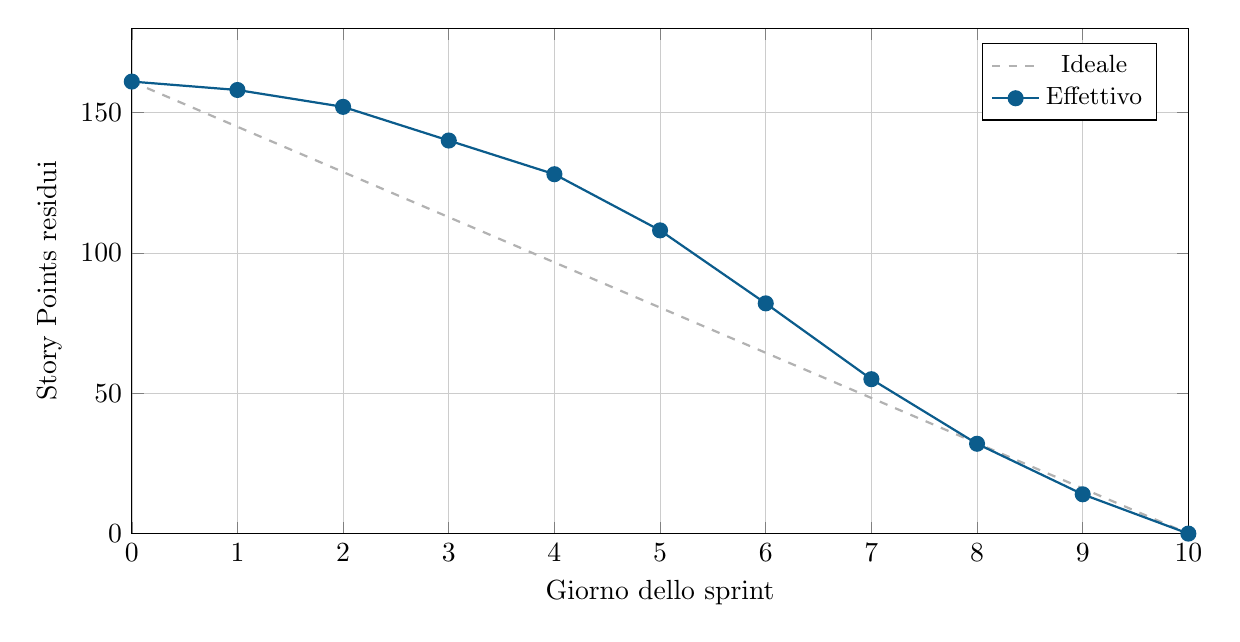
\begin{tikzpicture}
  \begin{axis}[
      width=15cm, height=8cm,
      xlabel={Giorno dello sprint}, ylabel={Story Points residui},
      xmin=0, xmax=10, ymin=0, ymax=180,
      xtick={0,1,2,3,4,5,6,7,8,9,10},
      grid=both,
      grid style={line width=.1pt, draw=gray!20},
      major grid style={line width=.2pt,draw=gray!40},
      legend pos=north east,
      legend style={font=\small},
  ]
  \addplot[color=gray!60, dashed, thick] coordinates {(0,161) (10,0)};
  \addlegendentry{Ideale}
  \addplot[color=accent, thick, mark=*, mark size=2.5pt] coordinates {
      (0,161) (1,158) (2,152) (3,140) (4,128)
      (5,108) (6,82)  (7,55)  (8,32)  (9,14) (10,0)
  };
  \addlegendentry{Effettivo}
  \end{axis}
  \end{tikzpicture}
  \end{center}

  % ------------------------------------------------------------------
  \subsection{API Design e implementazione back-end}
  % ------------------------------------------------------------------

  La specifica completa delle API \`{e} disponibile su Apiary all'indirizzo
  \url{https://trentoliveactivity.docs.apiary.io} e nel file \code{docs/openapi.yaml}
  all'interno del repository (circa 1940 righe, OpenAPI 3.0). In totale abbiamo
  documentato \textbf{72 endpoint} organizzati in \textbf{11 gruppi funzionali}. Tutti i route
  protetti richiedono un JWT firmato nell'header \code{Authorization: Bearer <token>};
  il controllo RBAC avviene a livello di middleware prima che la richiesta raggiunga
  il controller.

  La tabella seguente riporta gli endpoint principali per gruppo.

  \begin{small}
  \begin{longtable}{>{\centering\arraybackslash}p{1.6cm} p{7.2cm} p{6.2cm}}
  \toprule
  \rowcolor{headerBg}\color{white}\textbf{Metodo} & \color{white}\textbf{Path} &
  \color{white}\textbf{Descrizione breve} \\
  \midrule
  \endfirsthead
  \toprule
  \rowcolor{headerBg}\color{white}\textbf{Metodo} & \color{white}\textbf{Path} &
  \color{white}\textbf{Descrizione breve} \\
  \midrule
  \endhead
  %
  \multicolumn{3}{l}{\textbf{Autenticazione}} \\
  \midrule
  \rowcolor{rowAlt}POST & \code{/auth/register} & Registrazione cittadino (RF5, OCL C2/C5/C7) \\
  POST & \code{/auth/register/entity} & Registrazione ente certificato con PEC (RF31) \\
  \rowcolor{rowAlt}POST & \code{/auth/login} & Login; 2FA richiesto per AmministratoreDiSistema (RNF15) \\
  POST & \code{/auth/logout} & Revoca JWT corrente (inserisce in \code{RevokedToken}) \\
  \rowcolor{rowAlt}GET / PUT & \code{/auth/me} & Leggi o aggiorna profilo autenticato (RF20, RF13) \\
  DELETE & \code{/auth/me} & Cancellazione account (GDPR art.\ 17, RF26) \\
  \rowcolor{rowAlt}POST & \code{/auth/forgot-password} & Invio link reset password (RF8) \\
  POST & \code{/auth/reset-password/\{token\}} & Completamento reset password \\
  \rowcolor{rowAlt}POST & \code{/auth/2fa/setup} & Avvio setup 2FA TOTP per AmministratoreDiSistema \\
  POST & \code{/auth/2fa/verify} & Verifica e attivazione 2FA \\
  \midrule
  %
  \multicolumn{3}{l}{\textbf{Attivit\`{a}}} \\
  \midrule
  \rowcolor{rowAlt}GET & \code{/activities} & Lista attivit\`{a} attive (RF14, RF15, RF9) \\
  POST & \code{/activities} & Creazione attivit\`{a} spontanea (RF10, OCL C8--C11) \\
  \rowcolor{rowAlt}PUT & \code{/activities/\{id\}} & Modifica attivit\`{a} (solo creatore, OCL C12, RF19) \\
  DELETE & \code{/activities/\{id\}} & Annullamento attivit\`{a} (solo creatore) \\
  \rowcolor{rowAlt}POST & \code{/activities/\{id\}/join} & Iscrizione attivit\`{a} (RF11, OCL C13/C14/C18) \\
  DELETE & \code{/activities/\{id\}/join} & Cancellazione partecipazione (RF17, OCL C19) \\
  \rowcolor{rowAlt}GET & \code{/activities/\{id\}/calendar} & Export iCalendar (.ics) per attivit\`{a} (RF12, RF49) \\
  \midrule
  %
  \multicolumn{3}{l}{\textbf{Eventi certificati}} \\
  \midrule
  GET & \code{/events} & Lista eventi certificati (RF15) \\
  \rowcolor{rowAlt}POST & \code{/events} & Pubblicazione evento (RF21, OCL C15--C17, C24) \\
  GET & \code{/events/mine} & Eventi pubblicati dall'ente autenticato \\
  \rowcolor{rowAlt}PUT & \code{/events/\{id\}} & Modifica evento (solo ente pubblicante, RF24) \\
  GET & \code{/events/\{id\}/stats} & Statistiche evento (views, segnalazioni) per ente (RF25) \\
  \rowcolor{rowAlt}GET & \code{/events/\{id\}/calendar} & Export iCalendar (.ics) per evento (RF49) \\
  \midrule
  %
  \multicolumn{3}{l}{\textbf{Mappa e POI}} \\
  \midrule
  GET & \code{/map} & Dati mappa: POI + attivit\`{a} + eventi (RF2, RF3) \\
  \rowcolor{rowAlt}GET & \code{/map/geocode} & Reverse geocoding proxy verso Nominatim \\
  POST & \code{/map/poi} & Creazione POI -- solo AmministratoreDiSistema (RF36) \\
  \rowcolor{rowAlt}GET / PUT & \code{/map/poi/\{id\}} & Lettura o modifica POI \\
  DELETE & \code{/map/poi/\{id\}} & Eliminazione POI \\
  \midrule
  %
  \multicolumn{3}{l}{\textbf{Moderazione}} \\
  \midrule
  \rowcolor{rowAlt}POST & \code{/moderation/events/\{eventId\}/report} & Segnalazione evento (RF16, OCL C22/C23) \\
  GET & \code{/moderation/reports} & Lista segnalazioni -- AmministratoreDiSistema (RF33) \\
  \rowcolor{rowAlt}PATCH & \code{/moderation/reports/\{id\}} & Risoluzione segnalazione: \texttt{rimuovi} / \texttt{archivia} / \texttt{in\_lavorazione} (DSA, RNF23/24) \\
  \midrule
  %
  \multicolumn{3}{l}{\textbf{Admin e Dashboard}} \\
  \midrule
  GET & \code{/admin/entities/pending} & Enti in attesa di approvazione (RF31) \\
  \rowcolor{rowAlt}PATCH & \code{/admin/entities/\{id\}/approve} & Approvazione ente: imposta \code{approvato=true} \\
  PATCH & \code{/admin/entities/\{id\}/reject} & Rifiuto ente: elimina account \\
  \rowcolor{rowAlt}GET & \code{/admin/users} & Lista tutti gli utenti \\
  DELETE & \code{/admin/users/\{id\}} & Eliminazione utente (con cascata) \\
  \rowcolor{rowAlt}GET & \code{/dashboard/stats} & Statistiche aggregate -- AmministratoreComunale (RF27--29, OCL C25) \\
  GET & \code{/dashboard/stats/export} & Export statistiche in CSV o PDF (RF30) \\
  \midrule
  %
  \multicolumn{3}{l}{\textbf{Notifiche}} \\
  \midrule
  \rowcolor{rowAlt}POST & \code{/notifications/device-token} & Registrazione token FCM dispositivo (RF40) \\
  DELETE & \code{/notifications/device-token} & Deregistrazione token FCM \\
  \bottomrule
  \end{longtable}
  \end{small}

  \begin{tcolorbox}[callout]
  \textbf{Note implementative.}
  Tutti gli endpoint sono esposti tramite l'API Gateway (\code{backend/src/gateway/})
  che si occupa di validazione JWT, routing e rate limiting.
  I controller di ogni servizio (auth, activities, events, map, moderation, dashboard)
  sono separati in cartelle dedicate sotto \code{backend/src/}. L'autenticazione SPID per
  l'AmministratoreComunale \`{e} implementata come stub nell'endpoint \code{POST /auth/login}
  con un flag dedicato, in attesa dell'integrazione con il provider SPID reale.
  \end{tcolorbox}

  % ------------------------------------------------------------------
  \subsection{User Interface}
  % ------------------------------------------------------------------

  Il frontend \`{e} realizzato in \textbf{React + TypeScript} con Vite come bundler.
  Il design system \`{e} completamente custom (nessun framework CSS esterno), con un tema
  glass-morphism coerente in tutte le schermate. La mappa interattiva usa \textbf{MapLibre GL JS}
  con tile da OpenFreeMap. Di seguito descriviamo le schermate implementate per ciascun ruolo.

  \paragraph{Visitatore (non autenticato).}
  Il visitatore accede senza credenziali alla schermata principale che mostra la
  \textbf{mappa pubblica} (\code{MapPage}) con POI, attivit\`{a} ed eventi sovrapposti in
  layer separati. I marker si raggruppano in cluster al diminuire dello zoom; cliccando
  si apre un popup con i dettagli. \`{E} disponibile anche la \textbf{lista degli eventi
  certificati} (\code{EventsPage}) con card editoriali e banner dell'evento in evidenza,
  e la pagina di \textbf{dettaglio evento} (\code{EventDetailPage}). Le pagine di supporto
  includono \code{LoginPage}, \code{RegistrationPage} (con gate et\`{a} e consensi GDPR),
  \code{PasswordResetPage}, \code{VerifyEmailPage}, \code{TermsPage} e \code{PrivacyPage}.
  Queste schermate coprono prevalentemente US-01, US-02, US-03, US-26.

  \paragraph{Cittadino (UtenteRegistrato).}
  Dopo il login, il cittadino accede a tutte le funzionalit\`{a} sociali della piattaforma.
  La \textbf{mappa} (\code{MapPage}) si arricchisce di filtri aggiuntivi (``Per te'',
  ``Preferiti'') basati sugli interessi configurati nell'\textbf{onboarding}
  (\code{OnboardingInteressiPage}). La pagina \textbf{Attivit\`{a}} (\code{ActivitiesPage})
  mostra un banner con la prossima attivit\`{a}, una timeline raggruppata per giorno e le
  sezioni ``Le mie attivit\`{a}'' e ``Sto partecipando''; il dettaglio singolo
  \`{e} in \code{ActivityDetailPage}. Il cittadino pu\`{o} segnalare eventi dalla
  \code{EventsPage} (pulsante Segnala, DSA). Il \textbf{profilo} (\code{ProfilePage})
  permette la modifica di dati, interessi e impostazioni privacy. Le \textbf{impostazioni}
  (\code{SettingsPage}) includono gestione delle notifiche push. Queste schermate coprono
  US-07, US-11, US-12, US-13, US-16, US-17, US-21, US-23.

  \paragraph{Ente certificato (EnteCertificato).}
  L'ente approvato accede a \code{EntityPublishPage}, la schermata di creazione e
  gestione degli eventi certificati con supporto per badge di verifica, categoria,
  descrizione libera e allegati. Dalla stessa area pu\`{o} visualizzare le statistiche
  dei propri eventi (views e segnalazioni ricevute) tramite \code{EventDetailPage} con
  tab statistiche. L'ente \textbf{non pu\`{o}} segnalare i propri eventi attraverso il
  pulsante Segnala (il controllo \`{e} applicato lato frontend e backend).
  Queste schermate coprono US-09, US-15.

  \paragraph{Amministratore di sistema (AmministratoreDiSistema).}
  L'accesso richiede 2FA TOTP, configurato in \code{Setup2FAPage}. La \textbf{dashboard
  admin} comprende quattro aree principali: \code{AdminEntitiesPage} per la
  coda di approvazione/rifiuto degli enti (con invio automatico di email); \code{AdminUsersPage}
  per la gestione di tutti gli utenti con ricerca per ruolo e cancellazione con cascata;
  \code{AdminModerationPage} per la gestione delle segnalazioni DSA (stati
  \emph{aperta / in lavorazione / risolta}, con azione \emph{rimuovi} che elimina l'evento);
  \code{AdminPOIPage} per il CRUD dei Punti di Interesse sulla mappa con location picker
  integrato. Queste schermate coprono US-05, US-10, US-18, US-24, US-25.

  \paragraph{Amministratore comunale (AmministratoreComunale).}
  L'admin comunale accede tramite SPID (stub nel backend) a tre schermate dedicate.
  \code{ComuneDashboardPage} presenta le KPI principali (utenti, attivit\`{a}, eventi,
  POI, partecipazioni). \code{ComuneStatistichePage} offre grafici a barre per
  ``Attivit\`{a} per tipo'' e ``POI per affollamento'' con filtri per tipo, intervallo
  temporale e area geografica selezionabile tramite mappa interattiva (AreaMapPicker).
  \code{ComuneExportPage} consente di configurare i parametri di export (dataset, formato
  CSV/PDF, filtri) e di scaricare il file risultante. Queste schermate coprono
  US-19, US-20, US-33.

  % ------------------------------------------------------------------
  \subsection{Test cases (design)}
  % ------------------------------------------------------------------
  La tabella riporta i principali casi di test per area funzionale nel formato richiesto dal
  docente. I test sono implementati con \textbf{Jest} sul backend; la colonna \emph{Risultato
  effettivo} \`{e} compilata in fase di esecuzione.

  \begingroup
  \scriptsize
  \setlength{\tabcolsep}{2pt}
  \renewcommand{\arraystretch}{1.1}
  \begin{longtable}{p{0.9cm} p{1.1cm} p{2.6cm} p{3.0cm} p{1.8cm} p{1.0cm} p{2.4cm} p{0.9cm} p{1.3cm}}
  \toprule
  \rowcolor{headerBg}
  \color{white}\textbf{US} &
  \color{white}\textbf{N.} &
  \color{white}\textbf{Descrizione} &
  \color{white}\textbf{Dati test} &
  \color{white}\textbf{Precondizioni} &
  \color{white}\textbf{Dipend.} &
  \color{white}\textbf{Risultato atteso} &
  \color{white}\textbf{Ris. eff.} &
  \color{white}\textbf{Note} \\
  \midrule
  \endfirsthead
  \toprule
  \rowcolor{headerBg}
  \color{white}\textbf{US} &
  \color{white}\textbf{N.} &
  \color{white}\textbf{Descrizione} &
  \color{white}\textbf{Dati test} &
  \color{white}\textbf{Precondizioni} &
  \color{white}\textbf{Dipend.} &
  \color{white}\textbf{Risultato atteso} &
  \color{white}\textbf{Ris. eff.} &
  \color{white}\textbf{Note} \\
  \midrule
  \endhead
  %
  % ---- AUTENTICAZIONE ----
  US-02 & TC-A01 & Registrazione valida & POST /auth/register con email: mario@test.it, password: Password123!, dataNascita: 1995-06-15 & Nessun account con quella email & --- & 201 + emailVerification inviata & & --- \\
  \rowcolor{rowAlt}
  US-02 & TC-A02 & Registrazione et\`{a} $<$ 13 & POST /auth/register con dataNascita: 2020-01-01 & --- & --- & 400 AGE\_TOO\_YOUNG & & OCL C5 \\
  US-02 & TC-A03 & Email gi\`{a} registrata & POST /auth/register con email esistente & Account nel DB & TC-A01 & 409 EMAIL\_TAKEN & & OCL C7 \\
  \rowcolor{rowAlt}
  US-02 & TC-A04 & Login valido & POST /auth/login con email: mario@test.it, password: Password123! & Account verificato & TC-A01 & 200 + JWT & & --- \\
  US-02 & TC-A05 & Login password errata & POST /auth/login con password: Sbagliata1! & Account esistente & TC-A01 & 401 INVALID\_CREDENTIALS & & --- \\
  \rowcolor{rowAlt}
  US-05 & TC-A06 & Admin sistema senza OTP & POST /auth/login senza otpToken, utente con 2FA attivo & 2FA configurato & TC-A04 & 401 2FA\_REQUIRED & & RNF15 \\
  US-06 & TC-A07 & Reset password token scaduto & POST /auth/reset-password con token scaduto & Token nel DB & --- & 400 TOKEN\_EXPIRED & & RF8 \\
  \midrule
  %
  % ---- ATTIVIT\`{A} ----
  \rowcolor{rowAlt}
  US-11 & TC-AC01 & maxPartecipanti=1 (fuori range) & POST /activities con maxPartecipanti: 1 & Utente autenticato & --- & 400 INVALID\_MAX\_PARTECIPANTI & & OCL C8 \\
  US-11 & TC-AC02 & Data nel passato & POST /activities con data: 2024-01-01 & Utente autenticato & --- & 400 DATE\_IN\_PAST & & OCL C9 \\
  \rowcolor{rowAlt}
  US-11 & TC-AC03 & Creazione valida & POST /activities con tipo: sport, data futura, maxPartecipanti: 10 & Utente autenticato & --- & 201 + creator iscritto & & OCL C10 \\
  US-12 & TC-AC04 & Join doppio & POST /activities/:id/join, utente gi\`{a} iscritto & Partecipazione esistente & TC-AC03 & 409 ALREADY\_JOINED & & OCL C18 \\
  \rowcolor{rowAlt}
  US-12 & TC-AC05 & Attivit\`{a} piena & POST /activities/:id/join con attivit\`{a} al limite & maxPartecipanti raggiunto & TC-AC03 & 400 ACTIVITY\_FULL & & OCL C13 \\
  US-14 & TC-AC06 & Modifica da non-creatore & PUT /activities/:id da utente diverso & Attivit\`{a} nel DB & TC-AC03 & 403 FORBIDDEN & & OCL C12 \\
  \midrule
  %
  % ---- EVENTI ----
  \rowcolor{rowAlt}
  US-15 & TC-E01 & Ente non approvato & POST /events da ente con approvato: false & Ente non approvato nel DB & --- & 403 FORBIDDEN & & OCL C24 \\
  US-15 & TC-E02 & Titolo troppo lungo & POST /events con titolo di 101 caratteri & Ente approvato & --- & 400 INVALID\_TITLE & & OCL C17 \\
  \rowcolor{rowAlt}
  US-15 & TC-E03 & Pubblicazione valida & POST /events con titolo: Concerto, categoria: musica & Ente approvato & --- & 201 + badgeVerifica: true & & OCL C16 \\
  US-12 & TC-E04 & Join evento & POST /events/:id/join con JWT utente & Evento nel DB & TC-E03 & 200 + partecipazione registrata & & RF11 \\
  \midrule
  %
  % ---- MAPPA E POI ----
  \rowcolor{rowAlt}
  US-01 & TC-M01 & GET mappa pubblico & GET /map senza token & --- & --- & 200 + array markers & & RF2/RF3 \\
  US-24 & TC-M02 & POST POI da cittadino & POST /poi con JWT UtenteRegistrato & --- & --- & 403 & & RF36 \\
  \rowcolor{rowAlt}
  US-24 & TC-M03 & statoAffollamento non valido & POST /poi con statoAffollamento: blu & Admin autenticato & --- & 400 & & OCL C21 \\
  \midrule
  %
  % ---- MODERAZIONE ----
  US-17 & TC-MO01 & Segnalazione valida & POST /moderation/reports con tipo: spam, eventId valido & Utente autenticato & TC-E03 & 201 stato: aperta & & DSA \\
  \rowcolor{rowAlt}
  US-17 & TC-MO02 & Doppia segnalazione & POST /moderation/reports con stessa coppia userId+eventId & Segnalazione gi\`{a} presente & TC-MO01 & 409 ALREADY\_REPORTED & & OCL C22 \\
  US-18 & TC-MO03 & Risoluzione con rimozione & PATCH /moderation/reports/:id con azione: rimuovi & Segnalazione aperta, admin & TC-MO01 & 200 + evento rimosso & & RNF23/24 \\
  \midrule
  %
  % ---- DASHBOARD ----
  \rowcolor{rowAlt}
  US-19 & TC-D01 & Statistiche da admin comunale & GET /dashboard/stats con JWT AmministratoreComunale & --- & --- & 200 + dati aggregati & & OCL C25 \\
  US-19 & TC-D02 & Statistiche da cittadino & GET /dashboard/stats con JWT UtenteRegistrato & --- & --- & 403 & & OCL C25 \\
  \midrule
  %
  % ---- SICUREZZA ----
  \rowcolor{rowAlt}
  US-29 & TC-S01 & Token JWT scaduto & GET /activities con JWT scaduto & --- & --- & 401 TOKEN\_INVALID & & OWASP \\
  US-29 & TC-S02 & Token revocato post-logout & GET /activities con token in blacklist & Logout eseguito & TC-A04 & 401 TOKEN\_REVOKED & & RNF18 \\
  \rowcolor{rowAlt}
  US-28 & TC-S03 & Rate limiting su login & POST /auth/login ripetuto oltre soglia & --- & --- & 429 TOO\_MANY\_REQUESTS & & RNF \\
  \bottomrule
  \end{longtable}
  \endgroup

  \subsection{Sprint Review}
  La sprint review si \`{e} tenuta con tutti e tre i membri del team. Abbiamo mostrato i
  flussi principali per ogni ruolo: mappa pubblica con POI e affollamento, registrazione e
  login del cittadino (incluso OAuth Google), creazione di un'attivit\`{a} spontanea,
  pubblicazione evento da ente certificato, pannello admin di sistema con 2FA e moderazione
  DSA, e dashboard comunale con export CSV.

  I punti di forza emersi sono stati la coerenza tra il modello e l'implementazione sui
  vincoli OCL/GDPR e la completezza dei flussi di notifica. Le aree da migliorare riguardano
  la latenza al primo accesso e l'integrazione tra evento e POI sulla mappa. Per lo Sprint
  \#2 abbiamo deciso di prioritizzare il deploy live (US-34) e rimandare l'accessibilit\`{a}
  WCAG (US-30) a un'iterazione dedicata.

  \subsection{Product Backlog refinement}
  Sulla base di quanto emerso dalla sprint review, abbiamo aggiornato il backlog come segue.

  \paragraph{User story aggiunte:}
  \begin{itemize}
    \item \textbf{US-36}: Cleanup automatico dei \code{RevokedToken} scaduti (P2, 2~SP, S2).
    \emph{Emersa durante l'audit di sicurezza (T-32).}
    \item \textbf{US-37}: Vista calendario delle attivit\`{a}/eventi prossimi per il cittadino
    (P3, 5~SP, S2).
    \item \textbf{US-38}: Template HTML email escapati e branded (P2, 3~SP, S1, gi\`{a} chiuso
    in audit).
    \item \textbf{US-39}: Security headers (helmet, HSTS, CSP) (P2, 2~SP, S2).
  \end{itemize}

  \paragraph{User story modificate:}
  \begin{itemize}
    \item \textbf{US-19 (dashboard comunale)}: scope ridotto per evitare conteggi che
    identifichino singoli utenti. Il refactor \`{e} gi\`{a} stato mergiato.
    \item \textbf{US-34 (deploy)}: elevata a P1 in vista del D4.
  \end{itemize}

  \paragraph{User story rimosse / posticipate:}
  \begin{itemize}
    \item \textbf{US-30 (WCAG 2.1 AA)}: splittata in US-30a (audit accessibilit\`{a}) e
    US-30b (remediation), entrambe spostate allo Sprint \#2.
  \end{itemize}

  \subsection{Sprint Retrospective}

  \paragraph{\textcolor{accent2}{Cosa ha funzionato.}}
  La suddivisione del lavoro \`{e} stata efficace: ogni membro ha lavorato nell'area in cui
  aveva pi\`{u} esperienza (Filippo: backend e autenticazione; Saif: frontend e mappa; Anas: backend, notifiche, sicurezza, integrazione). Il workflow con feature branch e PR ha mantenuto il
  codice stabile. La suite di test ha intercettato alcune regressioni durante i refactor,
  confermando l'utilit\`{a} di averla scritta sin dall'inizio. L'audit di sicurezza a fine
  sprint ha prodotto 15 fix concreti e verr\`{a} replicato anche nel prossimo sprint.

  \paragraph{\textcolor{warn}{Cosa non ha funzionato.}}
  Alcuni task di integrazione tra frontend e backend hanno richiesto pi\`{u} tempo del previsto
  perch\'{e} i due layer erano stati sviluppati separatamente. La configurazione OAuth (consent
  screen, scope birthday, redirect URI) ha assorbito pi\`{u} ore del pianificato. Per lo
  Sprint \#2 puntiamo a PR pi\`{u} piccole e a usare una board GitHub Projects per tenere
  traccia dello stato dei task in modo pi\`{u} visibile.

  \paragraph{Obiettivi Sprint \#2.}
  Deploy live (US-34), accessibilit\`{a} WCAG (US-30), cleanup token revocati (US-36),
  security headers (US-39), calendario personale (US-37), copertura test frontend.

  \vspace{1cm}
  \begin{tcolorbox}[callout]
  \textbf{Conclusioni.} Lo Sprint \#1 ha superato le aspettative iniziali: 161~SP completati
  contro i 90~SP committati, con un'app effettivamente \emph{demo-ready} per tutti i 5 ruoli
  del modello D2. La qualit\`{a} di base \`{e} garantita da 69 test passanti al 100\%, un audit
  di sicurezza con 15 fix applicati e l'aderenza ai vincoli OCL e ai requisiti GDPR/DSA. Lo
  Sprint \#2 si concentrer\`{a} su deploy, accessibilit\`{a} e refinement della piattaforma.
  \end{tcolorbox}

\end{document}
